\documentclass[12pt,aspectratio=169]{beamer}

\usetheme[
    sectionpage=progressbar,
    subsectionpage=progressbar,
    progressbar=frametitle
]{metropolis}

\definecolor{mDarkBrown}{HTML}{FF5722}
\definecolor{mDarkTeal}{HTML}{263238}
\definecolor{mLightBrown}{HTML}{FF5722}

\usepackage{booktabs}
\usepackage{graphicx}
\usepackage{hyphenat}
\usepackage{multirow}
\usepackage[normalem]{ulem}

\usepackage{pifont}
\newcommand{\cmark}{\ding{51}}
\newcommand{\xmark}{\ding{55}}

\usepackage{polyglossia}
\setdefaultlanguage[variant=british]{english}
\usepackage[english=british]{csquotes}

\defaultfontfeatures{Ligatures=TeX}
\setmainfont{Lucida Sans OT}
\setsansfont[Scale=MatchLowercase]{Lucida Sans OT}
\setmonofont[Scale=MatchLowercase]{Lucida Console DK}

\author{Gianluca Campanella}
\date{}



\title{Introduction to machine learning}

\newcommand{\E}[1]{\ensuremath{\mathbb{E}\!\left[ #1 \right]}}
\newcommand{\V}[1]{\ensuremath{\mathbb{V}\!\left[ #1 \right]}}

\begin{document}

\maketitle

\begin{frame}{Contents}
    \tableofcontents[hideallsubsections]
\end{frame}

\section{Definitions}

\begin{frame}{Differences}
    \begin{block}{Statistics}
        \begin{itemize}
            \item Predates computers
            \item[$\rightarrow$] \textbf{Understand why something happens} in
                                 the face of uncertainty
        \end{itemize}
    \end{block}
    \vfill\pause
    \begin{block}{Machine Learning}
        \begin{itemize}
            \item `Algorithmic modelling' (L. Breiman)
            \item[$\rightarrow$] Computers can \textbf{learn rules} without
                                 explicit programming
        \end{itemize}
    \end{block}
\end{frame}

\begin{frame}{Two types of Data Science}
    \begin{columns}
        \begin{column}{0.5\textwidth}
            \begin{center}
                \large\bf%
                Analysis\hyp{}focused
            \end{center}
            \begin{itemize}
                \item Maths and Statistics
                \item Business Intelligence
                \item[$\to$] Assist human decision\hyp{}making
            \end{itemize}
        \end{column}
        \begin{column}{0.5\textwidth}
            \begin{center}
                \large\bf%
                Building\hyp{}focused
            \end{center}
            \begin{itemize}
                \item Machine Learning
                \item Software Engineering
                \item[$\to$] Develop and deploy data\hyp{}driven products
            \end{itemize}
        \end{column}
    \end{columns}
\end{frame}

\begin{frame}{The five questions}
    \begin{enumerate}
        \item How much/many?
        \item Is this A or B?
        \item How is this organised?
        \item Is this weird?
        \item What should I do next?
    \end{enumerate}
\end{frame}

\begin{frame}{How much/many?}
    \begin{block}{Examples}
        \begin{itemize}
            \item How many people will develop cancer in the next 10 years?
            \item How long will this patient stay in hospital?
        \end{itemize}
    \end{block}
    \begin{center}
        \large%
        $\downarrow$
        \vfill
        \textbf{Regression} algorithms
    \end{center}
\end{frame}

\begin{frame}{Is this A or B?}
    \begin{block}{Examples}
        \begin{itemize}
            \item How likely is this patient to be readmitted in the next year?
            \item What's the 10\hyp{}year CVD risk of this patient?
        \end{itemize}
    \end{block}
    \begin{center}
        \large%
        $\downarrow$
        \vfill
        \textbf{Classification} algorithms
    \end{center}
\end{frame}

\begin{frame}{How is this organised?}
    \begin{block}{Examples}
        \begin{itemize}
            \item Which patients develop similar diseases?
            \item Which diseases frequently occur together?
        \end{itemize}
    \end{block}
    \begin{center}
        \large%
        $\downarrow$
        \vfill
        \textbf{Clustering} algorithms
    \end{center}
\end{frame}

\begin{frame}{Is this weird?}
    \begin{block}{Examples}
        \begin{itemize}
            \item Is the number of cases higher than expected?
            \item Is this biomarker measurement abnormal?
        \end{itemize}
    \end{block}
    \begin{center}
        \large%
        $\downarrow$
        \vfill
        \textbf{Anomaly detection} algorithms
    \end{center}
\end{frame}

\begin{frame}{What should I do next?}
    \begin{block}{Examples}
        \begin{itemize}
            \item How should warfarin be dosed in this patient?
            \item How much insulin is needed to stabilise blood glucose?
        \end{itemize}
    \end{block}
    \begin{center}
        \large%
        $\downarrow$
        \vfill
        \textbf{Reinforcement learning} algorithms
    \end{center}
\end{frame}

\begin{frame}{Supervised vs unsupervised algorithms}
    \begin{columns}
        \begin{column}{0.5\textwidth}
            \begin{center}
                \large\bf%
                Supervised algorithms
            \end{center}
            \begin{itemize}
                \item Are trained on existing data
                \item Can be compared according to some `goodness' metric
            \end{itemize}
        \end{column}
        \begin{column}{0.5\textwidth}
            \begin{center}
                \large\bf%
                Unsupervised algorithms
            \end{center}
            \begin{itemize}
                \item Don't use examples with known outcomes
                \item Give clues, not `right answers'
            \end{itemize}
        \end{column}
    \end{columns}
\end{frame}

\begin{frame}{The five questions\ldots~revisited}
    \begin{center}
        \begin{tabular}{lll}
            \toprule
            \textbf{Family}               & \textbf{Class}         & \textbf{Question} \\
            \midrule
            \multirow{2}{*}{Supervised}   & Regression             & How much/many? \\
                                          & Classification         & Is this A or B? \\
            \midrule
            \multirow{2}{*}{Unsupervised} & Clustering             & How is this organised? \\
                                          & Anomaly detection      & Is this weird? \\
            \midrule
                                          & Reinforcement learning & What should I do next? \\
            \bottomrule
        \end{tabular}
    \end{center}
\end{frame}

\section{Prediction}

\begin{frame}{Guessing values}
    \begin{itemize}
        \item $Y$ = `length of hospital stay'
        \item You have some realisations $y_{1}, y_{2}, \ldots$ collected over
              time
        \item You want to predict the value of $Y$ for a new patient
    \end{itemize}
    \vfill\pause
    \begin{center}
        {\Large%
         How do you do this?} \\[1em]
        {If you prefer, what's the \textbf{optimal point forecast} for $Y$?}
    \end{center}
\end{frame}

\begin{frame}{Loss functions}
    Before you can answer, you need a \textbf{loss function} that\ldots
    \begin{itemize}
        \item Measures how big an error you're making with your guess $g$
        \item Can be minimised to obtain the `best' $g$
    \end{itemize}
    \vfill\pause
    \begin{center}
        \renewcommand*{\arraystretch}{1.5}
        \begin{tabular}{ll}
            \toprule
            \textbf{Mean squared error}  & $\operatorname{MSE}(g) = \E{ (Y - g)^{2}}$ \\
            \textbf{Mean absolute error} & $\operatorname{MAE}(g) = \E{ |Y - g|}$ \\
            \bottomrule
        \end{tabular}
    \end{center}
\end{frame}

\begin{frame}{Regression versus classification}
    \begin{block}{Regression}
        \begin{description}
            \item[Aim]  Predict a \textbf{continuous} value
            \item[Loss] How `off' (numerically) our predictions are
        \end{description}
    \end{block}
    \vfill
    \begin{block}{Classification}
        \begin{description}
            \item[Aim]  Predict a \textbf{class}
            \item[Loss] How `inaccurate' the predicted classes are
        \end{description}
    \end{block}
\end{frame}

\begin{frame}{Towards prediction\ldots}
    Usually we have at least another variable $X$ that we believe to be related
    to $Y$\ldots
    \vfill\pause
    \begin{block}{Idea}
        Using some function $f$ of $X$, we should be able to predict $Y$
        `\textbf{better}' (i.e.\ reduce the mean error) than by ignoring it
        \vfill
        \[
            g
            \;
            \leadsto
            \;
            f(X)
            \quad
            \text{and thus}
            \quad
            \operatorname{MSE}(f\,) = \E{(Y - f(X))^{2}}
        \]
    \end{block}
\end{frame}

\begin{frame}[t]{What should $f$ be?}
    \only<1>{%
        Consider the decomposition
        \[
            Y\,|\,X = f^{\,\star}(X) + \epsilon
        \]
        \begin{itemize}
            \item $f^{\,\star}$ is the optimal prediction (conditional on knowing $X$)
            \item $\epsilon$ is a random variable (since $f^{\,\star}$ is not)
            \item $\E{\epsilon} = 0$ without loss of generality
        \end{itemize}}
    \only<2>{%
        For the MSE, it can be shown that
        \[
            f^{\,\star}(x) = \E{ Y\,|\,X = x }
        \]
        \vfill
        $f^{\,\star}$ is what we'd like to know when we want to predict $Y$
        given $X$
        \begin{flushright}
            \ldots but can we?
        \end{flushright}}
\end{frame}

\section{Bias\hyp{}variance trade\hyp{}off}

\begin{frame}[t]{Bias\hyp{}variance trade\hyp{}off}
    \only<1>{%
        Suppose that\ldots
        \begin{itemize}
            \item The `true' regression function is $f^{\,\star}$
            \item We have to make do with some suboptimal $f$
        \end{itemize}
        \vfill
        Let's start by expanding the MSE\ldots
        \begin{align*}
            (Y - f \,)^{2}
            &= ( Y - f^{\,\star} + f^{\,\star} - f \,)^{2} \\
            &= [ ( Y - f^{\,\star} ) + ( f^{\,\star} - f \,) ]^{2} \\
            &= ( Y - f^{\,\star} )^{2}
               + 2 ( Y - f^{\,\star} ) ( f^{\,\star} - f \,)
               + ( f^{\,\star} - f \,)^{2}
        \end{align*}}
    \only<2>{%
        Now take the expectation\ldots
        \[
            \E{( Y - f^{\,\star} )^{2}
               + 2 ( Y - f^{\,\star} ) ( f^{\,\star} - f \,)
               + ( f^{\,\star} - f \,)^{2}}
        \]
        \vfill
        Since $Y - f^{\,\star} = \epsilon$ and $\E{\epsilon} = 0$, we have\ldots
        \begin{align*}
            \E{( Y - f^{\,\star} )^{2}} &= \V{\epsilon} \\
            \E{Y - f^{\,\star}} &= \E{\epsilon} = 0 \\
            \E{( f^{\,\star} - f \,)^{2}} &= ( f^{\,\star} - f \,)^{2}
        \end{align*}}
    \only<3>{%
        \[
            \E{\operatorname{MSE}(f\,)} = \alert{\V{\epsilon}} + ( f^{\,\star} - f \,)^{2}
        \]
        \vfill
        \begin{block}{Variance $\V{\epsilon}$}
            \begin{itemize}
                \item Doesn't depend on $f$, just on `how hard' it is to predict
                      $Y\,|\,X = x$
                \item[$\rightarrow$] Unpredictable, irreducible fluctuation
            \end{itemize}
        \end{block}}
    \only<4>{%
        \[
            \E{\operatorname{MSE}(f\,)} = \V{\epsilon} + \alert{( f^{\,\star} - f \,)^{2}}
        \]
        \vfill
        \begin{block}{Bias $( f^{\,\star} - f \,)^{2}$}
            \begin{itemize}
                \item `Extra error' we get from not knowing $f^{\,\star}$
                \item[$\rightarrow$] Amount by which we are systematically off
            \end{itemize}
        \end{block}}
    \only<5>{%
        Since $f$ is itself estimated from a sample (it's actually $\hat{f}\,$),
        we have\ldots
        \begin{itemize}
            \item The \textbf{irreducible variance} $\V{\epsilon}$
            \item The \textbf{bias} in approximating $f^{\,\star}$ using $f$
            \item The additional \textbf{(estimation) variance} of $\hat{f}$
        \end{itemize}
        \vfill
        \begin{block}{Consistent methods}
            \begin{itemize}
                \item Bias and estimation variance $\to 0$ as the sample size
                      increases
                \item Different consistent methods may converge at different
                      rates
            \end{itemize}
        \end{block}}
    \only<6>{%
        \begin{center}
            \vfill
            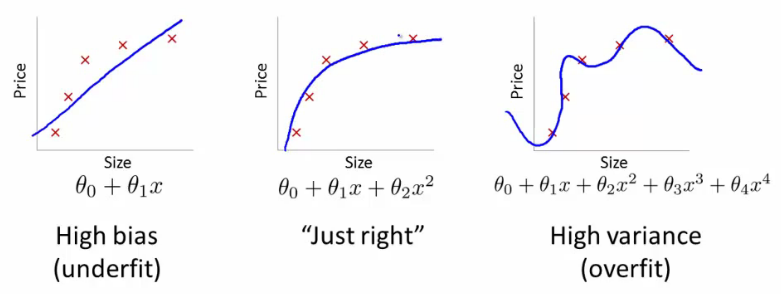
\includegraphics[width=\textwidth]{figures/underfitting_overfitting} \\[\bigskipamount]
            {\scriptsize%
             From Andrew Ng's \textit{Machine Learning} course}
            \vfill
        \end{center}}
\end{frame}

\begin{frame}{Bias\hyp{}variance trade\hyp{}off and generalisability}
    \begin{center}
        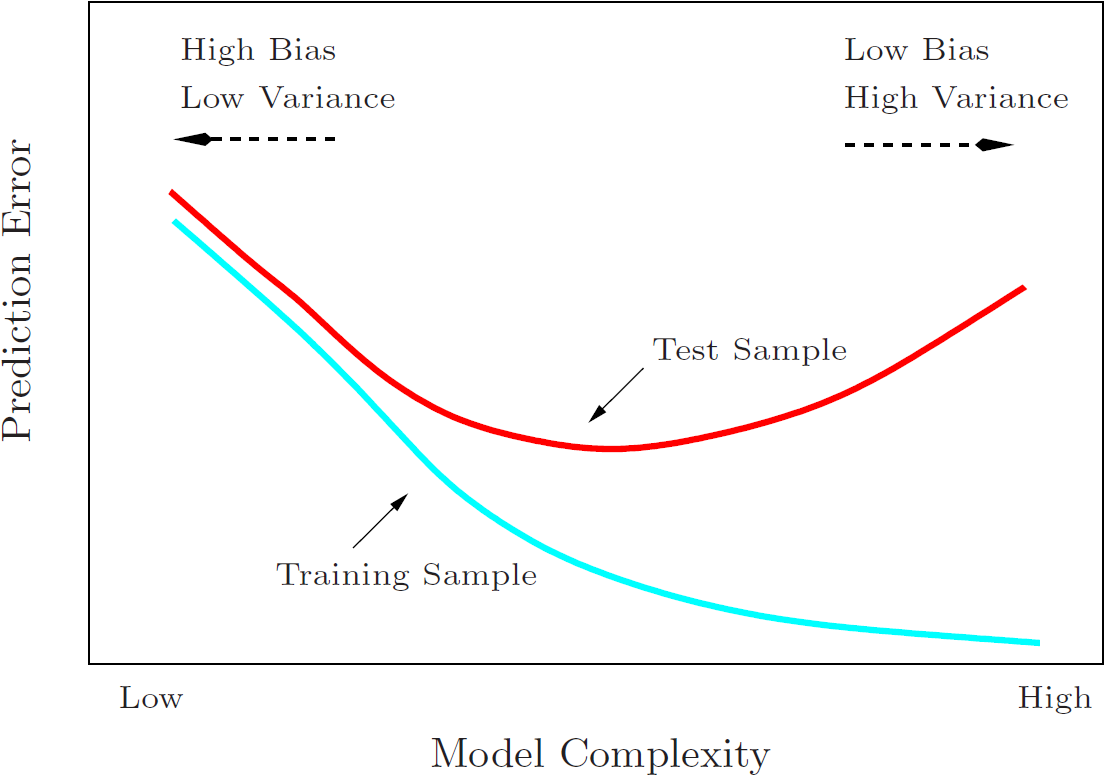
\includegraphics[height=0.8\textheight]{figures/generalisability} \\
        {\scriptsize%
         From \textit{The Elements of Statistical Learning}}
    \end{center}
\end{frame}

\begin{frame}{Cross\hyp{}validation}
    \begin{block}{General idea}
        \begin{itemize}
            \item Fit several models on subsets of the data
            \item Measure performance of each
            \item Compute the mean performance
        \end{itemize}
    \end{block}
\end{frame}

\begin{frame}{$k$-fold cross\hyp{}validation}
    \begin{itemize}
        \item Split the data into $k$ groups (a.k.a.\ `folds')
        \item Repeat for each fold:
              \begin{itemize}
                  \item Fit the model using all but the selected fold
                  \item Measure performance on the selected fold
              \end{itemize}
        \item Compute the mean performance across folds
    \end{itemize}
\end{frame}

\begin{frame}{Regularisation}
        \begin{itemize}
        \item Penalise `large' coefficients by shrinking them
        \item Helps avoid overfitting
        \item Requires \textbf{tuning} of an additional parameter $\alpha$
              representing the `weight' of the penalty (relative to the
              prediction error)
    \end{itemize}
    \vfill
    \begin{center}
        \renewcommand*{\arraystretch}{1.5}
        \begin{tabular}{lll}
            \toprule
            $L_{1}$ & LASSO & $\sum_{j} | \beta_{j} |$ \\
            $L_{2}$ & Tikhonov or ridge & $\sum_{j} \beta_{j}^{2}$ \\
            \bottomrule
        \end{tabular}
    \end{center}
\end{frame}

\end{document}

